\documentclass[french]{beamer}
\usefonttheme[onlymath]{serif}

\usepackage[utf8]{inputenc}
\usepackage[T1]{fontenc}
\usepackage{lmodern}
\usepackage{babel}

\usepackage{tikz}
\usepackage{pgfplots}
\usepackage{ifthen}

\usepackage{smartdiagram}
\usepackage[babel]{csquotes}
\usepackage[url=false, doi=false, style=science, backend=bibtex, bibencoding=ascii]{biblatex}
%\bibliography{IEEEabrv,bib/OAM}


\graphicspath{{img/}{../}}

\usepackage{../beamerthemeulaval}
\usepackage{../beamercolorthemeulaval}
\logo{\includegraphics[height=0.5cm]{UL_P}\hspace{.2cm}\vspace{.85\paperheight}}
\newcommand\red[1]{{\color{ulred}{\textbf{#1}}}}

\mode<presentation> {
	\setbeamercovered{invisible}
	\setbeamertemplate{navigation symbols}{} % Enlever les icônes de navigation
}

\title[Préparation]{Préparation des données}
%\subtitle[]{}

\author[C. Besse]{Camille Besse}
\institute[Université Laval]
{
	Départment d'Informatique et de Génie Logiciel\\
	Université Laval, Québec, Canada \\
	\medskip
	{\emph{camille.besse@ift.ulaval.ca}}
}
%\date{\today} % \today will show current date. 
% Alternatively, you can specify a date.


\AtBeginSection[]{
	\begin{frame}
	\Huge \centerline{\insertsection}
%  \small \tableofcontents[currentsection, hideothersubsections]
  \end{frame} 
}

\begin{document}



%----------------------------------------------------------------------------------------------------------------------------------------
\begin{frame}[label=titre, plain]
	\titlepage
	\begin{center}\includegraphics[height=1cm]{UL_P}\end{center}
\end{frame}


\section{Introduction}


%----------------------------------------------------------------------------------------------------------------------------------------

\input{../slprocess.tikz}


\begin{frame}[label=intro]{Introduction}
	\begin{center}
		\resizebox{\textwidth}{!}{
			\begin{tikzpicture}
			\only<1>{\pic {{slprocess}={1 and 1 and 1 and 1 and 1}};}
			\only<2->{\pic {{slprocess}={0 and 1 and 0 and 0 and 0}};}
			\end{tikzpicture}
		}	
	\end{center}
\end{frame}

%----------------------------------------------------------------------------------------------------------------------------------------
\begin{frame}{Introduction}
\begin{block}{Citation}
Les scientifiques de données ne travaillent que le \emph{\color{red}{vendredi}}

-- Anonyme
\end{block}
\end{frame}

\section*{Contents}

%----------------------------------------------------------------------------------------------------------------------------------------
\begin{frame}[label=toc]{Outline}
	\setlength{\leftskip}{5cm}%
	\tableofcontents[subsectionstyle=show]
\end{frame}



\section{Collecte \& Colligation}

\subsection{Principes essentiels}
%----------------------------------------------------------------------------------------------------------------------------------------
\begin{frame}{Collecte \& Colligation}
\begin{enumerate}
	\item Validité\\
	Cohérence et qualité de l'agrégation et de la colligation
	\item Fiabilité\\
	Procédure d'examen périodique et maintenance
	\item Temporalité\\
	Régularité des mesures et accessibilité en tout temps
	\item Précision\\
	Réduire au maximum les doublons ou les absents
	\item Intégrité\\
	Protection et/ou modification contrôlée
\end{enumerate} 
\end{frame}

\subsection{Nettoyage a priori}
%----------------------------------------------------------------------------------------------------------------------------------------
\begin{frame}{Nettoyage \textit{a priori}}
	\begin{itemize}
		\item Validation de la cohérence des colonnes/valeurs
		\item Validation de la cohérence colonnes/types
		\item Statistiques sur les colonnes\\
		Min/Max/Mean/Median cohérents
		\item Données manquantes en quelle proportion par ligne/colonne
		\item Quantité et signifiance des doublons ?
	\end{itemize} 
\end{frame}


\subsection{Erreurs courantes}
%----------------------------------------------------------------------------------------------------------------------------------------
\begin{frame}{Erreurs courantes à éviter}
\vspace{-1em}
	\begin{enumerate}
		\item Préparer sans objectif clair
		\item Préparer sans idée de visualiser
		\item Non contextualisation des données (éthique,culturel,\ldots)
		\item Saisie ou mauvaise transformation des données
		\item Analyse de (trop) peu de données
		\item Nommage confus des caractéristiques
		\item Duplication des données
		\item Altération des données
		\item Agrégation des sources
		\item Âgisme des données
	\end{enumerate} 
\end{frame}

\section[Outliers]{Données aberrantes}

%----------------------------------------------------------------------------------------------------------------------------------------
\begin{frame}{Nettoyage \textit{a priori}}
	\begin{itemize}
		\item Doit-on s'en préoccuper ?
		\begin{itemize}
			\item Dépend de la taille du dataset
		\end{itemize}
		\item S'il y a beaucoup de données : non.
		\item Si elles ont une influence sur une simple régression : peut-être. 
		\begin{itemize}
			\item Valider par visualisation.
		\end{itemize}	
		\item S'il y a peu de données: 
		\begin{itemize}
			\item Est-ce vraiment des données aberrantes ? 
			\item Ou juste des données débalancées ?
		\end{itemize}
		\item[$\Rightarrow$] Si possible : collecter toujours plus de données !
	\end{itemize}
\end{frame}

%----------------------------------------------------------------------------------------------------------------------------------------
\begin{frame}{Outliers}
	\begin{center}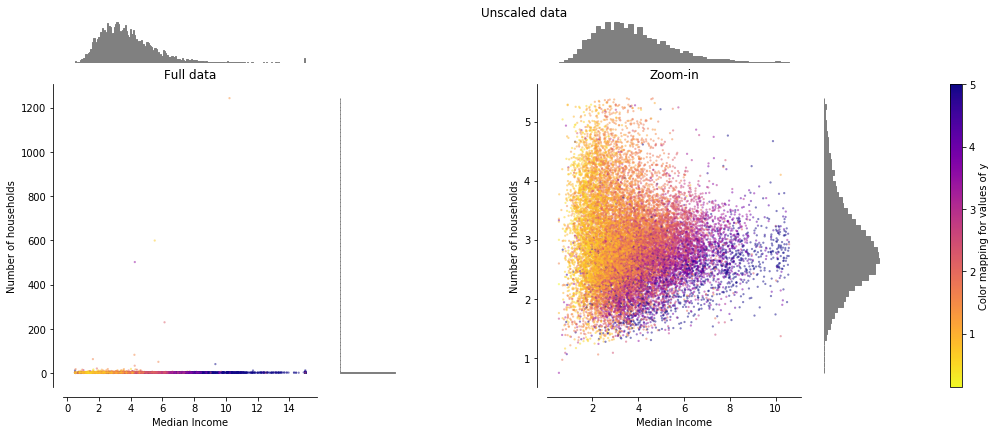
\includegraphics[width=\textwidth]{outliers.png}\end{center}
\end{frame}

%----------------------------------------------------------------------------------------------------------------------------------------
\begin{frame}{Identification}
	\begin{itemize}
		\item Covariance Robuste : Cherche la gaussienne qui explique le mieux les données 
		\begin{itemize}
			\item Sensible aux distributions multimodales
		\end{itemize}
		
		\item SVM mono-classe : séparateur a priori
		\begin{itemize}
			\item Bon pour déterminer la nouveauté mais sensible aux données aberrantes
		\end{itemize}		
		\item Forêt d'Isolation : random forest aléatoirement appris 
		\item Facteur local d'abérration : $k$-NN
	\end{itemize}
\end{frame}

\section[Imputation]{Données manquantes}

%----------------------------------------------------------------------------------------------------------------------------------------
\begin{frame}{Imputation}
Les données sont parfois incomplètes:
\begin{itemize}
	\item Certaines colonnes sont vides 
	\begin{itemize}
		\item Imputation
		\item On jette la donnée ? Combien de colonnes manquantes ? Cela change beaucoup les stats ?
	\end{itemize}
	
	\item Une colonne sans aucun sens pour les données
	\begin{itemize}
		\item Pas d'imputation (on jette la colonne ?)
	\end{itemize}		
\end{itemize}
\end{frame}

%----------------------------------------------------------------------------------------------------------------------------------------
\begin{frame}{Imputation}
\begin{itemize}
	\item Imputation simple : "\textit{Filling the blanks}"
	\begin{itemize}
		\item Statistiques : moyenne, mediane, selon la fréquence,\ldots
		\item Techniques non-paramétriques: k-nn, hot-deck (échantillonage de données similaires),\ldots
		\item Ou paramétriques: régression, \ldots
	\end{itemize}
	\item Imputation multiple: "\textit{Sampling the blanks}"
	\begin{itemize}
		\item Faire le travail plusieurs fois et évaluer l'impact statistique
	\end{itemize}		
\end{itemize}

\begin{center}
	\begin{Large}
		\textbf{\color{red}{FLAG}}
	\end{Large} \large\textbf{les données imputées pour éviter de les considérer comme des valeurs réelles !}
\end{center}
\end{frame}

\section[Unbalanced]{Données débalancées}

%----------------------------------------------------------------------------------------------------------------------------------------
\begin{frame}{Données débalancées}
\begin{itemize}
	\item Lorsque c'est plus simple de juste ignorer un sous-ensemble des données
	\begin{itemize}
		\item Qui se trouve être une catégorie complète \ldots
	\end{itemize}
	\item Solution 1 : Rééchantillonnage
	\begin{itemize}
		\item 	Synthetic Minority Oversampling TEchnique
		\begin{itemize}
			\item Bordeline : en privilégiant les frontières de décision
			\item Avec Boosting
		\end{itemize}
		\item Synthetic Majority Undersampling TEchnique (éventuellement informé)
		\begin{itemize}
			\item Cluster centroids : K-means
			\item Tomek Links
		\end{itemize}
	\end{itemize}		
\end{itemize}
\end{frame}

%----------------------------------------------------------------------------------------------------------------------------------------
\begin{frame}{Données débalancées}
\begin{itemize}
	\item Solution 2 : Algorithmes rebalancés par le coût
	\begin{itemize}
		\item La pénalité de mal classer un exemple de la classe minoritaire est plus grande que celui de l'autre classe
		\item[] e.g. Cost-sensitive boosting, decision trees ou neural networks
	\end{itemize}
	\item Solution 3 : Les deux techniques précédentes dans des méthodes à base de noyau ou par apprentissage actif
	\begin{itemize}
		\item[] e.g. Cost sensitive undersampling SVMs 
	\end{itemize}
	\item Autres : Classification mono-classe, métriques de rang plutôt que de classe.	
\end{itemize}
\end{frame}


\section[Norming]{Transformation des données}

%----------------------------------------------------------------------------------------------------------------------------------------
\begin{frame}{Transformation des données}
\begin{itemize}
	\item Rééchelonnage ([-1,1] or [0,1]) $$ x' = \frac{x-\min x}{\max x - \min x}$$
	\item Normalisation à la moyenne $$ x' = \frac{x- \bar{x}}{\max x - \min x}$$
	\item Standardisation (Loi de Gauss) $$ x' = \frac{x-\bar{x}}{\sigma_x}$$
	\item Normalisation à l'unité $$ x' = \frac{x}{|| x||}$$
\end{itemize}
\end{frame}


\subsection{Réduction de la dimensionalité}

	%----------------------------------------------------------------------------------------------------------------------------------------
\begin{frame}{Transformation des données}
	\begin{itemize}
		\item Projection d'un espace de taille $C$ dans un sous-espace de taille $n << C$
		\begin{itemize}
			\item Pour visualisation ($n=2$ ou $n=3$)
			\item Pour densifier l'information 
		\end{itemize}
		\item PCA, LDA, MDS, IsoMap, LLE, LTSA, t-NE,\ldots
	\end{itemize}

	\begin{center}
		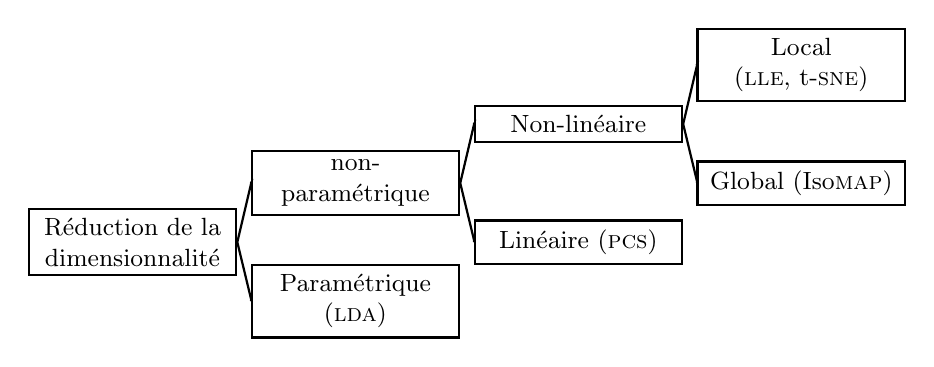
\begin{tikzpicture}[grow=right,edge from parent path={(\tikzparentnode.east) -- (.01,.01) -- (\tikzchildnode.west)}, thick]
		\tikzstyle{every node}=[align=center, draw=black,thick,anchor=west,text width=2.4cm,font=\small];
		\node {Réduction de la dimensionnalité}
			child { node {Paramétrique (\textsc{lda})}}		
			child { node {non-paramétrique}
				child { node {Linéaire (\textsc{pcs})}}
				child { node {Non-linéaire}
					child { node {Global (Iso\textsc{map})}}
					child { node {Local (\textsc{lle},~t-\textsc{sne})}}
					}
				};
		\end{tikzpicture}
	\end{center}
\end{frame}

%----------------------------------------------------------------------------------------------------------------------------------------
\begin{frame}{LDA : Linear Discriminant Analysis}
\begin{itemize}
	\item PCA dont l'objectif n'est pas de maximiser la variabilité, mais l'explicabilité d'une certaine variable catégorique (classe)
	\item Sélectionne les $n$ variables expliquant le mieux l'étiquette
\end{itemize}
\begin{center}
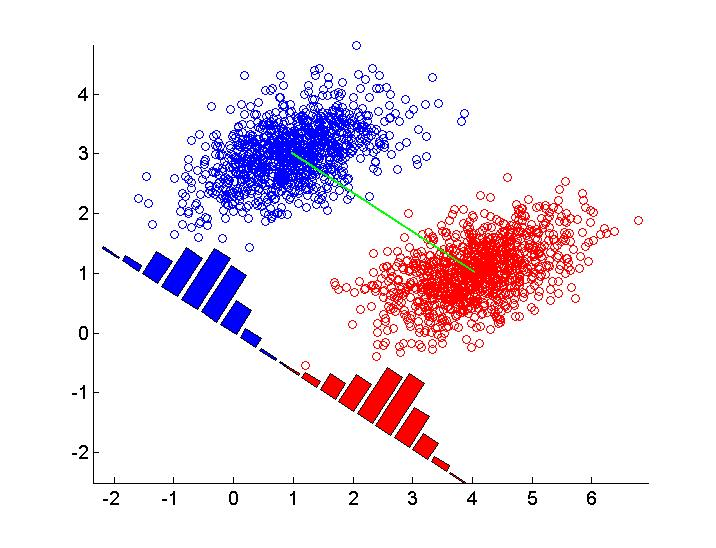
\includegraphics[width=0.7\textwidth]{lda}
\end{center}
\end{frame}


%----------------------------------------------------------------------------------------------------------------------------------------
\begin{frame}{MDS : Multi-Dimensionnal Scaling}
\begin{itemize}
	\item Généralisation du PCA sur  une mesure de dissimilarité entres les différents points
\end{itemize}
\begin{center}
	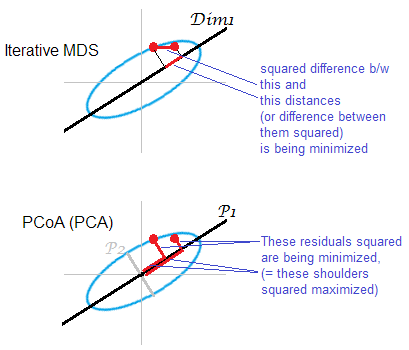
\includegraphics[width=0.7\textwidth]{mds}
\end{center}
\end{frame}

%----------------------------------------------------------------------------------------------------------------------------------------
\begin{frame}{IsoMAP}
\begin{itemize}
	\item MDS pour lequel on utilise une autre distance que la distance Euclidienne : Distance Géodesique
\end{itemize}
\begin{center}
	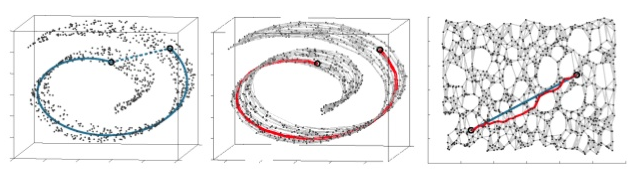
\includegraphics[width=\textwidth]{isomap}
\end{center}
\end{frame}

%----------------------------------------------------------------------------------------------------------------------------------------
\begin{frame}{LLE : Locally Linear Embedding}
\begin{itemize}
	\item Exprime un point selon une combinaison linéaire de ses voisins dans l'espace original
	$${E}(W) = \sum_i |\mathbf{X}_i - \sum_j \mathbf{W}_{ij}\mathbf{X}_j|^2$$
	\item Recalcul la position du point dans l'espace d'arrivée selon cette même combinaison 	
	$${C}(Y) = \sum_i |\mathbf{Y}_i - \sum_j \mathbf{W}_{ij}\mathbf{Y}_j|^2$$
\end{itemize}
\end{frame}

%----------------------------------------------------------------------------------------------------------------------------------------
\begin{frame}{LLE : Locally Linear Embedding}
\begin{center}
	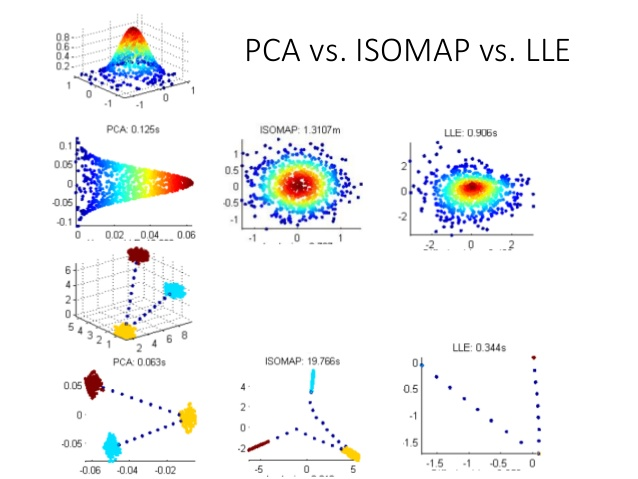
\includegraphics[width=.95\textwidth]{lle}
\end{center}
\end{frame}

%----------------------------------------------------------------------------------------------------------------------------------------
\begin{frame}{LTSA : Local Tangent Space Alignment}
\begin{itemize}
	\item Basée sur l'idée qu'un espace correctement "déplié" a tous ses hyperplans tangents alignés
	\item Calcule donc un hyperplan tangent pour chaque point calcule une représentation qui les aligne.
\end{itemize}
\begin{center}
	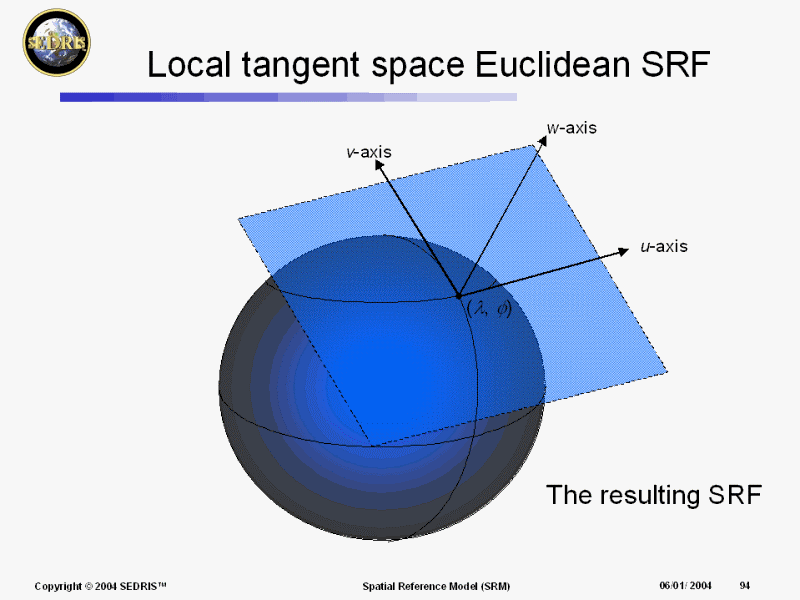
\includegraphics[width=0.7\textwidth]{ltsa}
\end{center}
\end{frame}

%----------------------------------------------------------------------------------------------------------------------------------------
\begin{frame}{t-SNE : t-distributed Stochastic Neighbour Embedding}
\begin{itemize}
	\item Transformation non linéaire des données dans un sous-espace de ou 3 dimensions
	\begin{itemize}
		\item Très souvent pour de la visualisation
	\end{itemize}
	\item Produit deux distributions de probabilité sur les paires de points proportionnelle à leur similarité:
	\begin{itemize}
		\item Dans l'espace à grand dimension
		\item Dans l'espace transformé
	\end{itemize}
	\item Minimise la KL-divergence entre les deux distributions selon leur position dans l'espace transformé
\end{itemize}
\end{frame}

%----------------------------------------------------------------------------------------------------------------------------------------
\begin{frame}{t-SNE : t-distributed Stochastic Neighbour Embedding}
\begin{center}
	\url{https://distill.pub/2016/misread-tsne/}
	
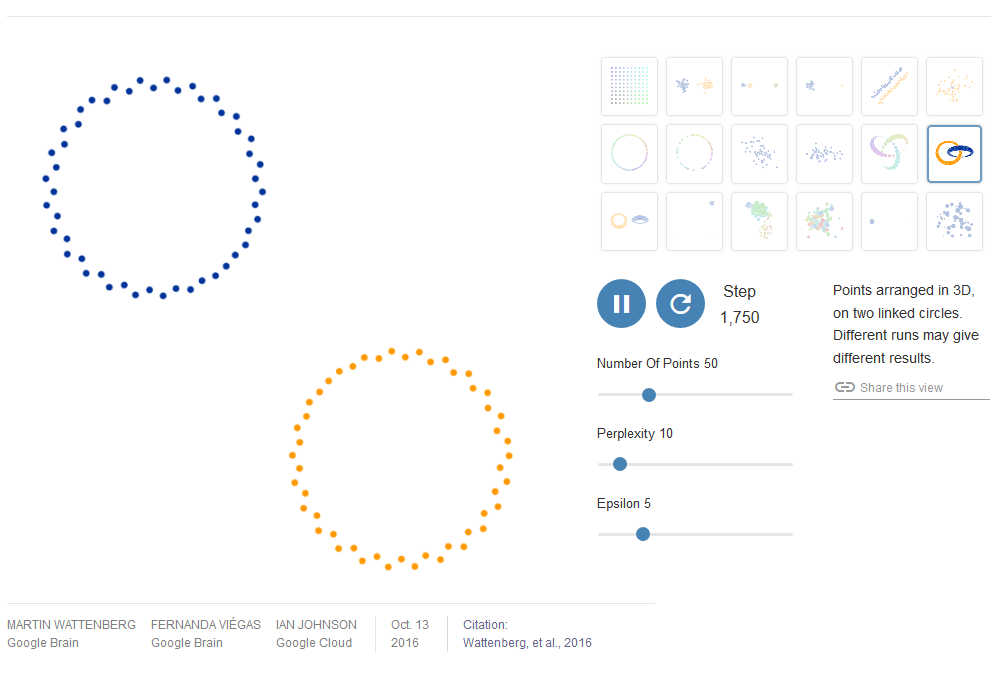
\includegraphics[width=.95\textwidth]{tsne}
\end{center}
\end{frame}


%----------------------------------------------------------------------------------------------------------------------------------------
\begin{frame}[label=conclu]{Conclusion}
	\begin{center}
		\Huge{That's all folks !}
	
		\normalsize Questions ?
	\end{center}
\end{frame}



% End of slides
\end{document}
